\documentclass[twocolumn]{article}
\usepackage[utf8]{inputenc}

\usepackage{tikz}
\usetikzlibrary{external}
\usetikzlibrary{shapes}
\usetikzlibrary{fit}

\usepackage{etoolbox} %for if empty functionality
\usepackage{leftidx}
\usepackage{ifthen}

\newcounter{a}
\newcounter{b}

\usepackage{ nopageno }

\usepackage{todonotes}

\usepackage{braket}

\usepackage{subcaption} % Subfigure environment 
\usepackage{gensymb}

\usepackage{amsmath} % Mathematical symbols
\usepackage{amssymb} % Symbols

\usepackage{caption}% Captions onder figuur gecentreerd
%\usepackage[toc,page]{appendix}
\usepackage{subcaption} % Subfigure environment 
\usepackage{float}

\usepackage{etoolbox} %for if empty functionality

\usepackage{ifthen}

%break long urls at a - and not only at . or /
\usepackage{url}
\def\UrlBreaks{\do\/\do-}
\usepackage{breakurl}
\usepackage[hidelinks,breaklinks]{hyperref}

\usepackage{verbatim}
\usepackage{cleveref}
\usepackage{amsfonts}
\usepackage{mathtools}

\usepackage{braket}
\usepackage{pdfpages}

\title{Cluster Expansion of Thermal States using Tensor
Networks}
\author{David Devoogdt}
\date{Academic year 2020-2021}


\begin{document}

\tikzset{add reference/.style={insert path={%
                    coordinate [pos=0,xshift=-0.5\pgflinewidth,yshift=-0.5\pgflinewidth] (#1 south west)
                    coordinate [pos=1,xshift=0.5\pgflinewidth,yshift=0.5\pgflinewidth]   (#1 north east)
                    coordinate [pos=.5] (#1 center)
                    (#1 south west |- #1 north east)     coordinate (#1 north west)
                    (#1 center     |- #1 north east)     coordinate (#1 north)
                    (#1 center     |- #1 south west)     coordinate (#1 south)
                    (#1 south west -| #1 north east)     coordinate (#1 south east)
                    (#1 center     -| #1 south west)     coordinate (#1 west)
                    (#1 center     -| #1 north east)     coordinate (#1 east)
                }}}
%\def\temp{#1}\ifx\temp\empty
%  <EMPTY>%
%\else
%  <NON EMPTY>%
%\fi

\newcommand{\combineTikz}[3]{
    \begin{tikzpicture}[baseline={0-0.5*height("$=$")}]
        \node (AA) at (0,0)  { #1   };
        \node (AB) at ( {#3} ,0)  {  #2  };
    \end{tikzpicture}
}

%\newcommand{\mpo}[6]  {\tikzexternalenable { \begin{tikzpicture}[baseline={0-0.5*height("$=$")}]
\newcommand{\mpo}[6]  { \begin{tikzpicture}[baseline={0-0.5*height("$=$")}]

        %\def \NNodes {#1}
        %\def \NodeName {#2}          
        %\def \NodeName {#2}          
        %\def \NodeName {#2}          
        %\def \NodeName {#2}          
        %\def \NodeName {#2}          
        %\def \NameUp   {#3} 
        %\def \NameUp   {#3} 
        %\def \NameUp   {#3} 
        %\def \NameUp   {#3} 
        %\def \NameUp   {#3} 
        %\def \NameDown  {#4}	
        %\def \NameDown  {#4}	
        %\def \NameDown  {#4}	
        %\def \NameDown  {#4}	
        %\def \NameDown  {#4}	

        \def \legLength {0.7}
        \def \radius {0.3}

        \pgfmathsetmacro{\step}{2*\radius+\legLength}
        \pgfmathsetmacro{\legpos}{\radius+\legLength}

        \pgfmathsetmacro{\Nmax}{#1-1}

        \foreach \N in {0,..., \Nmax }{
                \pgfmathsetmacro{\p}{\N*\step}

                % up and down labels
                \def\temp{#3}\ifx\temp\empty
                    \def \labelUp {}
                \else
                    \pgfmathsetmacro{\labelUp}{  {#3}[\N]  }
                \fi

                \def\tempp{#4}\ifx\tempp\empty
                    \def \labeldown {}
                \else
                    \pgfmathsetmacro{\labeldown}{  {#4}[\N]  }
                \fi

                \def\aab{#5}\ifx\aab\empty
                    \def \dotssite {0}
                \else
                    \pgfmathsetmacro{\dotssite}{  {#5}[\N]  }
                \fi

                \ifthenelse{\dotssite = 0}{

                    \def\aac{#6}\ifx\aac\empty
                        \def \nname {O}
                    \else
                        \pgfmathsetmacro{\nname}{  {#6}[\N]  }
                    \fi

                    \node[circle,draw, radius=\radius] (O\N) at (\p,0) {\nname};

                    \ifthenelse{ \equal{\labelUp}{-}  }{
                    }{
                        \node[] (Ou\N) at (\p, \legpos ) { \labelUp };
                        \draw (O\N) -- (Ou\N);
                    }

                    \ifthenelse{ \equal{\labeldown}{-}  }{
                    }{
                        \node[] (Od\N) at (\p,-\legpos) {\labeldown};
                        \draw (O\N) -- (Od\N);
                    }

                }{
                    \node[circle] (O\N) at (\p,0) { $\cdots$ };
                }

            }

        \ifthenelse{  #1  =1  }{}{
            \foreach \N in {1,...,\Nmax }{
                    \pgfmathsetmacro{\M}{\N-1}
                    \pgfmathsetmacro{\label}{ {#2}[\N]  }
                    %\pgfmathsetmacro{\label}{ 5}

                    \draw (O\M) --  node[above]  {\label} (O\N);
                }
        }

        \pgfmathsetmacro{\labelo}{ {#2}[0]}
        \pgfmathsetmacro{\labeli}{  {#2}[\Nmax+1]}

        \ifthenelse{ \equal{\labelo}{Tr}  }{

            \pgfmathsetmacro{\endpos}{\step*\Nmax+\radius}

            \draw plot [smooth ]  coordinates { (-\radius,0)    (-\radius, -0.45 )  (\endpos, -0.45)   (O\Nmax)   } ;
        }{
            \ifthenelse{ \equal{\labelo}{-}  }{
            }{
                \pgfmathsetmacro{\endpos}{\step*\Nmax+\legpos}

                \node (N0) at (-\legpos,0) {};
                \node (Ne) at (\endpos,0) {};

                \draw (N0) -- node[above] {\labelo} (O0);

                \draw (Ne) -- node[above] {\labeli}  (O\Nmax);
            }
        }
        %\draw (O0) --  node[above] {1} (O1);
        %\end{tikzpicture}} \tikzexternaldisable}
    \end{tikzpicture}}

%\newcommand{\expH}[5]{\tikzexternalenable { \begin{tikzpicture}[baseline={0-0.5*height("$=$")}]
\newcommand{\expH}[5]{\begin{tikzpicture}[baseline={0-0.5*height("$=$")}]
        \def \NNodes {#1};

        \def\aaa{#2}\ifx\aaa\empty
            \def \text { $e^{-\beta \hat{H}_{\NNodes} }$ }
        \else
            \def \text {#2}
        \fi

        \pgfmathwidth{ "\text" }
        \def \textwidth { \pgfmathresult }

        %\pgfmathsetmacro{\text}{width(\text)}

        \def \legLength {0.6}
        \def \radius {0.3} %fix to fit text inside for size 1
        \def \boxHeight {0.4};

        \pgfmathsetmacro{\step}{2*\radius+\legLength}
        \pgfmathsetmacro{\legpos}{\radius+\legLength}
        \pgfmathsetmacro{\dotpos}{\boxHeight+\legLength/2}

        \pgfmathsetmacro{\Nmax}{\NNodes -1}

        \pgfmathsetmacro{\boxsize}{ max ( \textwidth/1cm , \step*\Nmax )   + \radius}

        %\pgfmathsetmacro{\boxsize}{ 5  )}
        %\pgfmathsetlength{\boxsize}{ max( \textwidth,  \boxsize1  )}

        %            \ifthenelse{#1=1}{
        %                \def \left {-0.6}
        %                \def \right {0.6}
        %            }{
        \def \left {-\radius}
        \def \right {\boxsize}
        %            }

        \draw (\left,- \boxHeight ) rectangle (\right, \boxHeight ) [add reference =H] ;

        \node  at (H center) { \text };

        \foreach \N in {0,..., \Nmax }{
                \pgfmathsetmacro{\p}{\N*\step}

                % up and down labels
                \def\temp{#3}\ifx\temp\empty
                    \def \labelUp {}
                \else
                    \pgfmathsetmacro{\labelUp}{  {#3}[\N]  }
                \fi

                \def\tempp{#4}\ifx\tempp\empty
                    \def \labeldown {}
                \else
                    \pgfmathsetmacro{\labeldown}{  {#4}[\N]  }
                \fi

                \node[] (O\N) at (\p,0) {};

                \ifthenelse{ \equal{\labelUp}{...}  }{
                    \node[] (Ou\N) at (\p, \dotpos ) {\labelUp};
                }{
                    \ifthenelse{ \equal{\labelUp}{-}  }{

                    }{
                        \node[] (Ou\N) at (\p, \legpos ) {\labelUp};
                        \draw (Ou\N) --  (Ou\N  |- H north);
                    }
                }

                \ifthenelse{ \equal{\labeldown}{...}  }{
                    \node[] (Od\N) at (\p,-\dotpos ) {\labeldown};
                }{
                    \ifthenelse{ \equal{\labeldown}{-}  }{

                    }{
                        \node[] (Od\N) at (\p,-\legpos) {\labeldown};
                        \draw (Od\N) --  (Od\N  |- H south);
                    }
                }
            }

        \def\tempt{#5}\ifx\tempt\empty

        \else
            \pgfmathsetmacro{\labelo}{ {#5}[0] }
            \pgfmathsetmacro{\labeli}{  {#5}[1] }

            \pgfmathsetmacro{\leftleg}{  \left - \legLength }
            \pgfmathsetmacro{\rightleg}{  \right + \legLength }

            \node (N0) at (\leftleg,0) {\labelo};
            \draw (N0) -- ( N0  -| H west);

            \node (Ne) at (\rightleg,0) {\labeli};
            \draw (Ne) --  ( Ne  -| H east);
        \fi

        %        \end{tikzpicture}} \tikzexternaldisable }
    \end{tikzpicture} }

%\newcommand{\mpob}[6]  {\tikzexternalenable { \begin{tikzpicture}[baseline={0-0.5*height("$=$")},scale=0.8]
\newcommand{\mpob}[6]  {\begin{tikzpicture}[baseline={0-0.5*height("$=$")},scale=0.8]

        %\def \NNodes {#1}
        %\def \NodeName {#2}          
        %\def \NodeName {#2}          
        %\def \NodeName {#2}          
        %\def \NodeName {#2}          
        %\def \NodeName {#2}          
        %\def \NameUp   {#3} 
        %\def \NameUp   {#3} 
        %\def \NameUp   {#3} 
        %\def \NameUp   {#3} 
        %\def \NameUp   {#3} 
        %\def \NameDown  {#4}	
        %\def \NameDown  {#4}	
        %\def \NameDown  {#4}	
        %\def \NameDown  {#4}	
        %\def \NameDown  {#4}	

        \def \legLength {1.0}
        \def \radius {0.1}

        \pgfmathsetmacro{\step}{2*\radius+\legLength}
        \pgfmathsetmacro{\legpos}{\radius+\legLength}

        \pgfmathsetmacro{\Nmax}{#1-1}

        \foreach \N in {0,..., \Nmax }{
                \pgfmathsetmacro{\p}{\N*\step}

                % up and down labels
                \def\temp{#3}\ifx\temp\empty
                    \def \labelUp {}
                \else
                    \pgfmathsetmacro{\labelUp}{  {#3}[\N]  }
                \fi

                \def\tempp{#4}\ifx\tempp\empty
                    \def \labeldown {}
                \else
                    \pgfmathsetmacro{\labeldown}{  {#4}[\N]  }
                \fi

                \def\aab{#5}\ifx\aab\empty
                    \def \dotssite {0}
                \else
                    \pgfmathsetmacro{\dotssite}{  {#5}[\N]  }
                \fi

                \def\aac{#6}\ifx\aac\empty
                    \def \nname { "O" }
                \else
                    \pgfmathsetmacro{\nname}{  {#6}[\N]  }
                \fi

                %\node[] (O\N) at (\p,0) {\nname};
                \node[circle,draw, radius=\radius] (O\N) at (\p,0) {\nname};

            }

        \ifthenelse{  #1  =1  }{}{
            \foreach \N in {1,...,\Nmax }{
                    \pgfmathsetmacro{\M}{\N-1}
                    \pgfmathsetmacro{\label}{ {#2}[\N]  }
                    %\pgfmathsetmacro{\label}{ 5}

                    \draw (O\M) --  node[above]  {\label} (O\N);
                }
        }

        % \pgfmathsetmacro{\labelo}{ {#2}[0]}
        % \pgfmathsetmacro{\labeli}{  {#2}[\Nmax+1]}

        % \node (N0) at (-\legpos,0) {};
        % \draw (N0) -- node[above] {\labelo} (O0);

        % \pgfmathsetmacro{\endpos}{\step*\Nmax+\legpos}

        % \node (Ne) at (\endpos,0) {};
        % \draw (Ne) -- node[above] {\labeli} (O\Nmax);

        %\draw (O0) --  node[above] {1} (O1);

        % \end{tikzpicture}} \tikzexternaldisable}

    \end{tikzpicture}}

% \newcommand{\pepob}[5]  { \tikzexternalenable {\begin{tikzpicture}[baseline={0-0.5*height("$=$")},scale=0.8]
% \newcommand{\pepob}[5]  { \begin{tikzpicture}[baseline={0-0.5*height("$=$")},scale=1,
\newcommand{\pepob}[5]  { \begin{tikzpicture}[
            baseline={([yshift= -2ex ]current bounding box.north)},
            %baseline={0-0.5*height("$=$")},
            scale=1,
            Al/.style = {regular polygon, regular polygon sides=3,
                    draw, fill=white, text width=0.1,
                    inner sep=1mm, outer sep=0mm,
                    shape border rotate=-90},
            Ar/.style = {regular polygon, regular polygon sides=3,
                    draw, fill=white, text width=0.1,
                    inner sep=1mm, outer sep=0mm,
                    shape border rotate=90},
            Acc/.style = {diamond, draw, inner sep=1mm},
            Ac/.style = {rectangle, draw, inner sep=2mm}]

        %\pgfmathsetmacro{\llegLength}{ 0.3 }

        \def \legLength { 0.8}
        \def \radius {0.1}

        %\pgfmathtruncatemacro{\llegLength} { 0.8 }
        %\pgfmathtruncatemacro{\radius} { 0.1 }

        %\pgfmathtruncatemacro{\legLength}{2* \llegLength}
        %\pgfmathtruncatemacro{\lstep}{\radius+ \llegLength}
        %\pgfmathtruncatemacro{\step}{2*\lstep}
        \pgfmathsetmacro{\step}{2*\radius+ \legLength}

        \pgfmathsetmacro{\legpos}{\radius+\legLength}

        \pgfmathsetmacro{\Nmax}{#1-1}
        \pgfmathsetmacro{\Mmax}{#2-1}

        % define positions of different O's

        \setcounter{a}{0}
        %\setcounter{a}{0}

        \foreach \N in {0,..., \Nmax }{

                %\pgfmathtruncatemacro{\a}{\thea}

                \pgfmathsetmacro{\p}{  (\N + \thea) *\step   }
                %\setcounter{b}{0}

                \foreach \M in {0,..., \Mmax }{

                        %\pgfmathsetmacro{\p}{ \pp + \theb *\step   }

                        \pgfmathsetmacro{\k}{   \M   *\step  }

                        \pgfmathtruncatemacro{\s}{\M*(\Nmax+1)+\N   }

                        \pgfmathsetmacro{\nname}{ ""  }

                        \def\aab{#5}\ifx\aab\empty
                            \def \so {0}
                        \else
                            \pgfmathsetmacro{\so}{  {#5}[\s]  }
                        \fi

                        \ifthenelse{\so = 0}{
                            \node[circle,draw, radius=\radius] (O\s) at (\p,\k) {\nname};
                        }

                        \ifthenelse{\so = 2}{
                            \node[draw, Al] (O\s) at (\p,\k) {\nname};
                        }

                        \ifthenelse{\so = 3}{
                            \node[draw, Ar] (O\s) at (\p,\k) {\nname};
                        }

                        \ifthenelse{\so = 4}{
                            \node[draw= none, inner sep=0, outer sep=0 , minimum size=0pt] (O\s) at (\p,\k) {\nname};
                        }

                        \ifthenelse{\so = 6}{
                            \node[draw, Acc] (O\s) at (\p,\k) {\nname};
                        }

                        \ifthenelse{\so = 7}{
                            \node[draw, Ac] (O\s) at (\p,\k) {\nname};
                        }

                        %Gl environment
                        \ifthenelse{\so = 5}{

                            \pgfmathsetmacro{\recl}{  \p + \step - 3*\radius  }
                            \pgfmathsetmacro{\recr}{  \p + \step + 3*\radius  }

                            \pgfmathsetmacro{\recu}{  \k + 2*\radius }
                            \pgfmathsetmacro{\recd}{  \k - \step -2*\radius  }

                            % \pgfmathsetmacro{\recl}{  \p  +\step   }
                            % \pgfmathsetmacro{\mw}{ 2*\radius }
                            % \pgfmathsetmacro{\mh}{ \step  }

                            % \pgfmathsetmacro{\recu}{  \k - \step /2 }

                            % \node[rectangle,
                            %     draw,
                            %     minimum height= 1,
                            %     anchor=center  ] (O\s) at (\recl,\recu) {Gl};

                            \draw  (\recl,\recu) rectangle node[  ] (O\s)  {Gl}   (\recr,\recd)     ;

                            %\draw node[fill, minimum width= 1  ,minimum height= 1 ] (O\s) at (\recl,\recu) {Gl};
                            \stepcounter{a}
                        }

                        \ifthenelse{\so = 8}{

                            \node[draw, Ar] (O\s) at (\p,\k) {\nname};

                            \pgfmathtruncatemacro{\t}{\M*(\Nmax+1)+\N +1  }

                            \pgfmathsetmacro{\recl}{  \p +\step  - 3*\radius  }
                            \pgfmathsetmacro{\recr}{  \p + \step+  3*\radius  }

                            \pgfmathsetmacro{\recu}{  \k + 2*\radius }
                            \pgfmathsetmacro{\recd}{  \k - \step -2*\radius  }

                            \draw  (\recl,\recu) rectangle node (O\t)  {Gr}   (\recr,\recd)     ;

                            \draw  (O\s) -- (   O\t.west   |-  O\s  ) ;
                            \stepcounter{a}
                        }

                        \ifthenelse{\so = 9}{

                            \node[draw, Ac] (O\s) at (\p,\k) {\nname};

                            \pgfmathtruncatemacro{\t}{\M*(\Nmax+1)+\N +1  }

                            \pgfmathsetmacro{\recl}{  \p +\step  - 3*\radius  }
                            \pgfmathsetmacro{\recr}{  \p + \step+  3*\radius  }

                            \pgfmathsetmacro{\recu}{  \k + 2*\radius }
                            \pgfmathsetmacro{\recd}{  \k - \step -2*\radius  }

                            \draw  (\recl,\recu) rectangle node (O\t)  {Gr}   (\recr,\recd)     ;

                            \draw  (O\s) -- (   O\t.west   |-  O\s  ) ;
                            \stepcounter{a}
                        }

                        \ifthenelse{\so = 10}{

                            \node[draw = none] (O\s) at (\p,\k) {\nname};

                            \pgfmathtruncatemacro{\t}{\M*(\Nmax+1)+\N +1  }

                            \pgfmathsetmacro{\recl}{  \p +\step  - 3*\radius  }
                            \pgfmathsetmacro{\recr}{  \p + \step+  3*\radius  }

                            \pgfmathsetmacro{\recu}{  \k + 2*\radius }
                            \pgfmathsetmacro{\recd}{  \k - \step -2*\radius  }

                            \draw  (\recl,\recu) rectangle node (O\t)  {Gr}   (\recr,\recd)     ;

                            \draw  (O\s) -- (   O\t.west   |-  O\s  ) ;
                            \stepcounter{a}
                        }

                        \ifthenelse{\so = 11}{

                            \node[draw , Acc] (O\s) at (\p,\k) {\nname};

                            \pgfmathtruncatemacro{\t}{\M*(\Nmax+1)+\N +1  }

                            \pgfmathsetmacro{\recl}{  \p +\step  - 3*\radius  }
                            \pgfmathsetmacro{\recr}{  \p + \step+  3*\radius  }

                            \pgfmathsetmacro{\recu}{  \k + 2*\radius }
                            \pgfmathsetmacro{\recd}{  \k - \step -2*\radius  }

                            \draw  (\recl,\recu) rectangle node (O\t)  {Gr}   (\recr,\recd)     ;

                            \draw  (O\s) -- (   O\t.west   |-  O\s  ) ;
                            \stepcounter{a}
                        }

                        \ifthenelse{\so = 12}{

                            \node[circle,draw, radius=\radius] (O\s) at (\p,\k) {\nname};

                            \pgfmathsetmacro{\pp}{   \p+\legLength/2 }
                            \pgfmathsetmacro{\pm}{   \p-\legLength/2  }

                            \pgfmathsetmacro{\kp}{   \k+\legLength/2  }
                            \pgfmathsetmacro{\km}{   \k-\legLength/2  }

                            \node (Op\s) at (\pp,\kp) {i};
                            \node (Om\s) at (\pm,\km) {j};

                            \draw (O\s.center)  --  (Op\s);
                            \draw  (Om\s) --  (O\s);
                        }

                        \ifthenelse{\so = 13}{

                            \node[draw= none] (O\s) at (\p,\k) { ... };
                        }

                        \ifthenelse{\so = 14}{

                            \node[circle,draw, radius=\radius] (O\s) at (\p,\k) {\nname};

                            \pgfmathsetmacro{\pp}{   \p+\legLength/2 }
                            \pgfmathsetmacro{\pm}{   \p-\legLength/2  }

                            \pgfmathsetmacro{\kp}{   \k+\legLength/2  }
                            \pgfmathsetmacro{\km}{   \k-\legLength/2  }

                            \node (Op\s) at (\pp,\kp) {};
                            \node (Om\s) at (\pm,\km) {};

                            \draw (O\s.center)  --  (Op\s);
                            \draw  (Om\s) --  (O\s);
                        }

                        \ifthenelse{\so = 15}{

                            \node[circle,draw, radius=\radius] (O\s) at (\p,\k) {\nname};

                            \pgfmathsetmacro{\pp}{   \p+\legLength/2 }

                            \pgfmathsetmacro{\kp}{   \k+\legLength/2  }

                            \node (Op\s) at (\pp,\kp) {};

                            \draw (O\s.center)  --  (Op\s);
                        }

                        \ifthenelse{\so = 16}{
                            \node[draw, Ac] (O\s) at (\p,\k) {B};
                        }

                        \ifthenelse{\so = 17}{
                            \node[circle,draw=none, radius=\radius] (O\s) at (\p,\k) {\nname};
                        }

                        \ifthenelse{\so = 18}{

                            \node[circle,draw=none, radius=\radius] (O\s) at (\p,\k) {\nname};

                            \pgfmathtruncatemacro{\t}{\M*(\Nmax+1)+\N +1  }

                            \pgfmathsetmacro{\recl}{  \p +\step  - 3*\radius  }
                            \pgfmathsetmacro{\recr}{  \p + \step+  3*\radius  }

                            \pgfmathsetmacro{\recu}{  \k + 2*\radius }
                            \pgfmathsetmacro{\recd}{  \k - \step -2*\radius  }

                            \draw  (\recl,\recu) rectangle node (O\t)  {Gr}   (\recr,\recd)     ;

                            \draw  (O\s) -- (   O\t.west   |-  O\s  ) ;
                            \stepcounter{a}
                        }

                        \ifthenelse{\so = 22}{
                            \node[draw,line width=0.6mm  ,Al] (O\s) at (\p,\k) {};
                        }

                        \ifthenelse{\so = 23}{
                            \node[draw,line width=0.6mm  ,Ar] (O\s) at (\p,\k) {};
                        }

                        \ifthenelse{\so = 25}{
                            \node[draw,line width=0.6mm ,Ac] (O\s) at (\p,\k) {};
                        }

                        \ifthenelse{\so = 24}{
                            \node[draw, Ac] (O\s) at (\p,\k) {Fl};
                        }

                        \ifthenelse{\so = 26}{
                            \node[draw, Ac] (O\s) at (\p,\k) {Fr};
                        }

                    }
            }

        %connect nodes horizontally with correct name
        \foreach \M in {0,..., \Mmax }{
                \foreach \N in {1,...,\Nmax}{

                        \pgfmathtruncatemacro{\s}{\M*(\Nmax+1)+\N   }

                        \pgfmathtruncatemacro{\t}{\M*(\Nmax+1)+\N  -1 }

                        \pgfmathtruncatemacro{\l}{\M*(\Nmax)+\N -1 }

                        %\pgfmathsetmacro{\label}{ {#2}[\N]  }
                        %\pgfmathsetmacro{\label}{ \l }
                        \pgfmathsetmacro{\label}{ {#3}[\l]  }

                        \def\aab{#5}\ifx\aab\empty
                            \def \so {0}
                        \else
                            \pgfmathsetmacro{\so}{  {#5}[\s]  }
                        \fi

                        \def\aab{#5}\ifx\aab\empty
                            \def \to {0}
                        \else
                            \pgfmathsetmacro{\to}{  {#5}[\t]  }
                        \fi

                        \ifthenelse{ \equal{\label}{Gl}  }{

                            \pgfmathtruncatemacro{\ogl}{ (\M+1)*(\Nmax+1)+\N -1 }

                            \draw (O\ogl.east   |- O\s  )  --  (O\s);

                            \draw (O\t)  --  ( O\ogl.west    |-  O\t  );

                        }{

                            \ifthenelse{ \equal{\label}{Gr}  }{

                                \pgfmathtruncatemacro{\ogl}{ (\M+1)*(\Nmax+1)+\N  }

                                \draw (O\t)  --  ( O\ogl.west    |-  O\t  );

                                \draw (O\ogl.east   |- O\s  )  --  (O\s);

                            }{

                                \ifthenelse{ \NOT  \so = 1  }{
                                    \ifthenelse{ \NOT  \to = 1}{
                                        \ifthenelse{ \equal{\label}{-} }{

                                        }
                                        {

                                            \draw ( O\t.east |- O\s )  --  node[above]  {\label} (O\s);
                                        }
                                    }
                                }
                            }

                        }

                    }
            }

        %connect nodes vertically with correct name
        \foreach \N in {0,...,\Nmax }{
                \foreach \M in {1,..., \Mmax }{

                        \pgfmathtruncatemacro{\s}{\M*(\Nmax+1)+\N   }

                        \pgfmathtruncatemacro{\t}{ (\M-1)*(\Nmax+1)+\N  }

                        \pgfmathtruncatemacro{\l}{\N*\Mmax+\M  -1 }

                        %\pgfmathsetmacro{\label}{ {#4}[\l]  }
                        \pgfmathsetmacro{\label}{ {#4}[\l]  }

                        \def\aab{#5}\ifx\aab\empty
                            \def \so {0}
                        \else
                            \pgfmathsetmacro{\so}{  {#5}[\s]  }
                        \fi

                        \def\aab{#5}\ifx\aab\empty
                            \def \to {0}
                        \else
                            \pgfmathsetmacro{\to}{  {#5}[\t]  }
                        \fi

                        % \pgfmathtruncatemacro{\st}{ \so+\to  }

                        % \ifthenelse{\st = 0}{
                        %     \draw (O\t) --  node[left]  {\label} (O\s);
                        % }

                        \ifthenelse{ \( \NOT  \so = 1 \) \AND \( \NOT  \so = 5 \) }{
                            \ifthenelse{ \NOT  \to = 1}{
                                \ifthenelse{ \equal{\label}{-} }{

                                }
                                {
                                    \draw (O\t) --  node[left]  {\label} (O\s);
                                }
                            }
                        }

                    }
            }

        % \pgfmathsetmacro{\labelo}{ {#2}[0]}
        % \pgfmathsetmacro{\labeli}{  {#2}[\Nmax+1]}

        % \node (N0) at (-\legpos,0) {};
        % \draw (N0) -- node[above] {\labelo} (O0);

        % \pgfmathsetmacro{\endpos}{\step*\Nmax+\legpos}

        % \node (Ne) at (\endpos,0) {};
        % \draw (Ne) -- node[above] {\labeli} (O\Nmax);

        %\draw (O0) --  node[above] {1} (O1);

        % \pgfmathsetmacro{\s}{\Nmax*\step+0.5}
        % \pgfmathsetmacro{\t}{\Mmax*\step+0.5}

        % \draw[draw=none] (-0.5,-0.5) |- (\s,\t) |- cycle;

        %\end{tikzpicture}} \tikzexternaldisable}
    \end{tikzpicture}}



\maketitle

\begin{abstract}
    There is a theory which states that if ever anyone discovers exactly what the Universe is for and why it is here, it will instantly disappear and be replaced by something even more bizarre and inexplicable.
There is another theory which states that this has already happened.
\end{abstract}

\section{Introduction}

\section{Tensor Networks}

Matrix Product States (MPS) form an ansatz to describe the
\begin{equation}
    \ket{\Psi} = \sum_{i_1 i_2 \cdots i_n } C^{i_1 i_2 \cdots i_n} \ket{i_1} \otimes \ket{i_2} \otimes \cdots \otimes \ket{i_n}
\end{equation}
The tensor C needs $d^n$ numbers to describe the full wave function. In uniform MPS, the tensor $ C^{i_1 i_2 \cdots i_n}$ is subdivided into the product of n tensors $C$ and a matrix $M$ that contains the boundary conditions
\begin{equation} \label{c_split}
    C^{i_1 i_2 \cdots i_n} = Tr( C^{i_1} C^{i_2} \cdots C^{i_n} M  ).
\end{equation}
If M is the identity matrix, the chain is closed cyclically. Tensor networks are typically denoted in their graphical form (see \cref{tab:grafical_not}). External lines denote free indices, connected lines implies a summation over the shared line, analogous to matrix multiplication.
\begin{table}[]
    \centering
    \caption{Examples of graphical notation.}
    \begin{tabular}{l|l|l}
        conventional            & Einstein                & tensor notation           \\
        \hline
        $\Vec{x}$               & $x_{\alpha}$            &

        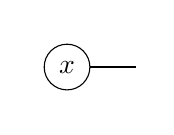
\begin{tikzpicture}[baseline=({N2.base}) ]
            \clip (-0.5,-0.5) rectangle (1,0.5);
            \node[circle, draw] (N2) at (0,0) {$x$};
            \node[] (N1) at (1,0) {};
            \draw  (N1) -- (N2) ;
        \end{tikzpicture}                                                     \\
        M                       & $M_{\alpha \beta}$      & 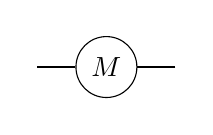
\begin{tikzpicture}[baseline={0cm-0.5*height("$=$")} ]
            \clip (-1,-0.5) rectangle (1,0.5);

            \node[circle, draw] (N2) at (0,0) {$M$};
            \node[] (N0) at (-1,0) {};
            \node[] (N1) at (1,0) {};

            \draw  (N1) -- (N2) ;
            \draw  (N0) -- (N2) ;

        \end{tikzpicture} \\

        $\Vec{x} \cdot \Vec{y}$ & $x_{\alpha} y_{\alpha}$ & 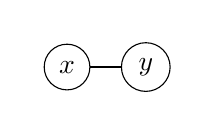
\begin{tikzpicture}[baseline=({N2.base}) ]
            \clip (-0.5,-0.5) rectangle (1.5,0.5);
            \node[circle, draw] (N2) at (0,0) {$x$};
            \node[circle, draw] (N1) at (1,0) {$y$};
            \draw  (N1) -- (N2) ;
        \end{tikzpicture} \\
    \end{tabular}

    \label{tab:grafical_not}
\end{table}
\Cref{c_split} is in this graphical notation becomes
\begin{equation}\label{eq:general_mps}
    \mpo{5}{{"Tr",,,,,}}{{"$i_1$","$i_2$",,"$i_n$","-"}}{{"-","-",,"-","-"}}{{0,0,1,0,0}}{{"C", "C",,"C","M" }}.
\end{equation}
An MPS has 2 dimension, the physical dimnsion of the particles $d = dim \left( \ket{i_2}  \right)$ and the dimension $\chi$ of the bonds between the tensors. The cluster expansion will rely on "virtual levels". This is the division of the MPS in blocks, analogous to dividing a matrix into block matrices. Every virtual level has its own associated dimension
\subsection{MPO}
A matrix procuct operator (MPO), is similar to an MPS but has 2 physical legs $i$ and $j$. The following compact notation is used in this paper
\begin{equation}
    O^{0 0} = \mpo{1}{ {0,0}  }{ {"$i$",}  }{ {"$j$",}}{}{{"",}} = \mpob{1}{ {0,0}  }{ {"$i$",}  }{ {"$j$",}}{}{{"",}}.
\end{equation}
This is the MPO with virtual level 0 and physical indices $i$ and $j$, which will both be omitted. Non-zero virtual indices are shown, and summation over virtual level is implied. Summation over shared virtual bond 1 on 2 neighbouring sites is denoted as
\begin{equation}
    O^{0 1} O^{1 0} = \mpob{2}{ {0,1,0}  }{ {"$i_1$","$i_2$"}  }{ {"$j_1$","$j_1$",}}{}{{"",}}.
\end{equation}
While contraction over all possible virtual levels on 3 sites is denoted by
\begin{equation} \label{PEPO_3}
    \mpob{3}{ {0,,,0}  }{}{}{}{{"",,}} .
\end{equation}

\section{Strongly correlated matter}

\subsection{Transversal Ising}

\begin{figure}[h!]
    \center
    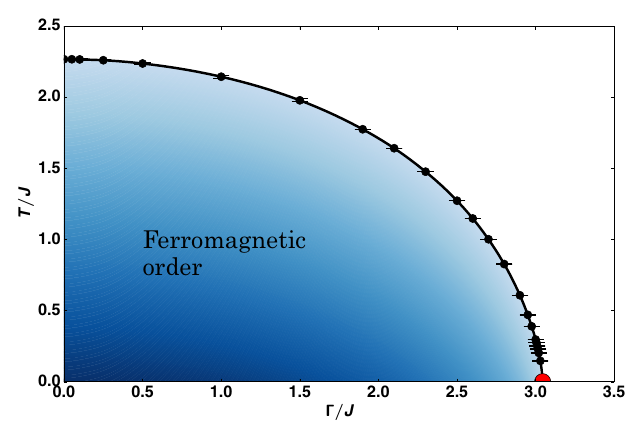
\includegraphics[width=\linewidth]{../Figuren/phsyics/2disingphase.png}
    \caption{Phase diagram for 2D transversal Ising model. Figure taken from \cite{Hesselmann2016}.}
    \label{2dtisingphasediag}
\end{figure}

\subsection{Criticality}

\subsection{operator exponentials}

\subsection{TN contraction}

\section{Cluster Expansion}

The novel method to construct a PEPO $e^{-\beta \hat{H}}$ with cluster expansions. An example is given by \cref{PEPO_3}.  This was first introduced in \cite{Vanhecke2021}. The goal is capture the exponential of the Hamiltonian operator $\hat{H}$
\begin{equation}
    \hat{H} = \left (  \sum_{<i j>} H^i_2 H^j_2 + \sum_i H^i_1 \right )
\end{equation}
This Hamiltonian consists of 1 and 2 site operators. Of course more general Hamiltonians can also be used. The notation for the contraction of the tensor network will also be used to denote the Hamiltonian evaluated on the given geometry
\begin{alignat}{3}
    H \left( \mpob{3}{ {0,,,0}  }{}{}{}{{"",,}} \right ) = & H_1 &  & \otimes 1   &  & \otimes 1  \nonumber  \\
    +                                                      & 1   &  & \otimes H_1 &  & \otimes 1 \nonumber   \\
    +                                                      & 1   &  & \otimes 1   &  & \otimes H_1 \nonumber \\
    +                                                      & H_2 &  & \otimes H_2 &  & \otimes 1   \nonumber \\
    +                                                      & 1   &  & \otimes H_2 &  & \otimes H_2 \nonumber \\.
\end{alignat}

\subsection{Idea}

The main idea is to make an extensive expansion by adding blocks which solve the model exactly on a local patch. Crucially, the expansion is not in the inverse temperature $\beta$ but in the size of the patches. The local patches are separated by a virtual level 0 bond. To make this somewhat more precise, the first steps of the expansion are shown here. The smallest patch, i.e. 1 site,  encodes the exponential of that Hamiltonian
\begin{equation}
    \mpob{1}{ {0,0}  }{}{}{}{{"",}} = \exp \left( -\beta H(\mpob{1}{}{}{}{}{{"",}})   \right).
\end{equation}
If there were no 2 site interactions, this already captures the full diagonalisation. Of course, such a model wouldn't be useful. The next step is to introduce 2 site interactions, where the one site interactions are subtracted from the diagonalised Hamiltonian.
\begin{equation} \label{eq:lev1}
    \begin{split}
        \mpob{2}{ {0,1,0}  }{}{}{}{{"",}}  = \exp -\beta H( & \mpob{2}{ {,,} }{}{}{}{{"",}})  \\
        - &\mpob{2}{ {0,0,0}  }{}{}{}{{"",}}
    \end{split}
\end{equation}
Contraction of larger network lead to many terms, such as
\begin{equation}
    \mpob{10}{ {0,1,0,0,0,1,0,1,0,0,1,0}  }{}{}{}{{"","","","","","","","","","","",}} .
\end{equation}
The beauty of this lays in the fact that disconnected regions(regions separated by level 0) combine in exactly the right way to capture the terms appearing in the series expansion of the exact tensor exponential. \cite{Vanhecke2021} Only the terms of the exponential which acts on 3 or more neighbouring sites at once, are not accounted for.

Notice that in \cref{eq:lev1}, 2 new blocks are introduced. The dimension of virtual level 1 needs to be $d^2$, with d the dimension of physical level. Although different possible constructions, already differ in the next step, one more step is added to make te construction and notation clear.
\begin{equation}\label{constr:intro:gen}
    \begin{split}
        \mpob{3}{ {0,1,1,0}  }{}{}{}{{,,,}}  = \exp  -\beta H( &\mpob{3}{ {,,,} }{}{}{}{{,,}})  \\
        - \;&\mpob{3}{ {0,0,0,0}  }{}{}{}{{,,,}}\\
        - \; &\mpob{3}{ {0,1,0,0}  }{}{}{}{{,,,}}\\
        - \; &\mpob{3}{ {0,0,1,0}  }{}{}{}{{,,,}}\\[3pt]
        =\exp  -\beta H( &\mpob{3}{ {,,,} }{}{}{}{{,,}})\\[3pt]
        - \; &\mpob{3}{ {,,,}  }{}{}{}{{,,,}}\\
    \end{split}
\end{equation}
This is called an cluster expansion of order 3, because there are 3 connected sites solved exactly. The right-hand side of \cref{constr:intro:gen} can be ommited, as it is just evaluating the exponentiated Hamiltonian on the same geometry as the left hand side and substructing all possible contractions of the blocks which were added previously. This very compact notation will be able to capture the essence of the different constructions. Because it is important for the remainder of the chapter, it is stressed that for an equation similar to
\begin{equation}
    \boxed{\mpob{3}{ {0,1,1,0}  }{}{}{}{{,,,}} },
\end{equation}
the right-hand side of \cref{constr:intro:gen} is implied. In the following section, different types will be discussed. For every chain lenght, a new block is defined. This could be done in numerous ways. The different types will be discussed in the next sections.

\subsection{1D}
\subsubsection{Type A}
The first few blocks in the cluster expansion are
\begin{subequations}
    \begin{align}
         & \mpob{1}{ {,}  }{}{}{}{{,,}}                      \\
         & \mpob{2}{ {,"1",}  }{}{}{}{{,,}}                  \\
         & \mpob{3}{ {,"1","1",}  }{}{}{}{{,,,}}             \\
         & \mpob{4}{ {,"1","2","1",}  }{}{}{}{{,,,,,}}       \\
         & \mpob{5}{ {,"1","2","2","1",}  }{}{}{}{{,,,,,}} .
    \end{align}
\end{subequations}
Virtual level $l$ needs a bond dimension of $d^{2 l}$ to solve the equations.  The introduction of $O^{n n}$ blocks lead to long chains. This could result in diverging behaviour for cyclic systems.

\subsubsection{Type E}
To remedy this behaviour, type E only has these blocks
\begin{subequations}
    \begin{align}
         & \mpob{1}{ {,}  }{}{}{}{{,,}}                       \\
         & \mpob{2}{ {,"1",}  }{}{}{}{{,,}}                   \\
         & \mpob{3}{ {,"1","1'",}  }{}{}{}{{,,,}}             \\
         & \mpob{4}{ {,"1","2","1'",}  }{}{}{}{{,,,,,}}       \\
         & \mpob{5}{ {,"1","2","2'","1'",}  }{}{}{}{{,,,,,}}.
    \end{align}
\end{subequations}
The bond dimension $\chi$ is twice as large, because for every virtual level there is also a primed level. With these blocks, it is impossible to make a patch longer than what is solved explicitly. This generalises well to higher dimension.

\subsubsection{Type F}
Both type A and F have potentially ill conditioned inverses. The blocks of type F are
\begin{subequations}
    \begin{align}
         & \mpob{1}{ {,}  }{}{}{}{{,,}}                                          \\
         & \mpob{2}{ {,"1'",}  }{}{}{}{{,,}}+  \mpob{2}{ {,"1'",}  }{}{}{}{{,,}} \\
         & \mpob{3}{ {,"1","1",}  }{}{}{}{{,,,}}                                 \\
         & \mpob{4}{ {,"1","2","1",}  }{}{}{}{{,,,,,}} \; +  \nonumber           \\
         & \mpob{4}{ {,"1","2'","1",}  }{}{}{}{{,,,,,}}                          \\
         & \mpob{5}{ {,"1","2","2","1",}  }{}{}{}{{,,,,,}} .
    \end{align}
\end{subequations}

The blocks $O^{n n+1}$ are unitary up to a constant factor. The primed blocks solve the chains of even order. This requires twice the bond dimension of type A, but is guaranteed to have well conditioned inverses.

\subsection{2D}
In hindsight of the results, the construction in 2D is a generalisation of type A. The linear blocks, which are given by a tree graph, will be a direct generalisation. The non-linear blocks are used to account for loops.
\subsubsection{Linear}
The generalisation of an MPO to 2D is called a PEPO (project entangle pair operator). These PEPO's are graphically depicted by the same symbol
\begin{equation}
    \mpob{1}{ {,}  }{}{}{}{{,,}} = \vcenter{ \hbox{ \pepob{4}{3}{{
                        "-","-","-",
                        "-","0","0",
                        "-","-","-"}}{{
                        "-","-",
                        "-","-",
                        "0","0",
                        "-","-"}}{{
                        1,1,4,1,
                        1,4,12,4,
                        1,1,4,1}} }}.
\end{equation}
The construction starts of as
\begin{equation}\label{2dblocksorder2}
    \pepob{2}{2}{{"1",,}}{{,,}}{{0,0,1,1}}  \quad   \pepob{2}{2}{{,,}}{{"1",,}}{{0,1,0,1}}.
\end{equation}
For the order 3 blocks, 6 different options are possible. They are
\begin{equation}
    \pepob{2}{2}{{"1","1",}}{{"1","1",}}{{0,0,0,1}} \;
    \pepob{3}{2}{{"1","1","1","1"}}{{"1","1","1","1"}}{{0,0,0,1,1,1}}
\end{equation}
and rotations over 90 degrees. Solving all blocks such that
\begin{equation}
    \vcenter{ \hbox{ \pepob{4}{3}{{
                        "-","-","-",
                        "-","a","c",
                        "-","-","-"}}{{
                        "-","-",
                        "-","-",
                        "d","b",
                        "-","-"}}{{
                        1,1,4,1,
                        1,4,12,4,
                        1,1,4,1}} }} = \vcenter{ \hbox{ \pepob{4}{3}{{
                        "-","-","-",
                        "-","b","d",
                        "-","-","-"}}{{
                        "-","-",
                        "-","-",
                        "a","c",
                        "-","-"}}{{
                        1,1,4,1,
                        1,4,12,4,
                        1,1,4,1}} }}
\end{equation}
reduced the number of blocks that need to be solved significantly. Also T and + blocks should be added
\begin{equation}\label{crosssolve}
    \pepob{3}{2}{{"1","1","1","1"}}{{"1","1","1","1"}}{{0,0,0,1,0,1}} \quad   \pepob{3}{3}{{"1","1","1","1","1","1",}}{{"1","1","1","1","1","1",}}{{1,0,1,0,0,0,1,0,1}}.
\end{equation}
From here on, it can again be generalised to longer chains and +'s. Care has to be taken to construct the blocks in the right order.

\subsubsection{Nonlinear}
Not all finite size patches are covered with the blocks introduced in the previous section. The lowest order block not covered is
\begin{equation}\label{tikzfig:plaquetter}
    {\pepob{2}{2}{{"$\alpha$","$\alpha$",}}{{"$\alpha$","$\alpha$",}}{{0,0,0,0}}}.
\end{equation}
This is a nonlinear equation, and will be treated separatey in \cref{sec:solv}. All virtual levels for solving loops are denoted by Greek letters. For $d=2$, the bond dimension of $\alpha$ can be as low as 6. To connect the loops to the linear blocks, corner pieces similar to
\begin{equation}\label{eq:loop_1ext}
    \pepob{5}{3}{{
                "-","-", "-",     "-",
                "-","1","$\beta$","-",
                "-","-","$\alpha$","-"}}{{
                "-","-",
                "-","-",
                "-","$\gamma$",
                "-","$\alpha$",
                "-","-"}}{{
                1,1,1,1,1,
                1,0,0,0,1,
                1,1,0,0,1}}
\end{equation}
are used. Directly connecting to $O^{ \alpha \alpha 0 1 }$ also solves the local patch, but cause diverging results when 2 or more corner pieces with extensions connect. One corner can connect to 2 chains, with length of the same order as the linear blocks. Going further is possible, comes at an ever increasing bond dimension cost.

\subsection{Solvers} \label{sec:solv}

\subsubsection{Linear Solver}

\def \pepoct { 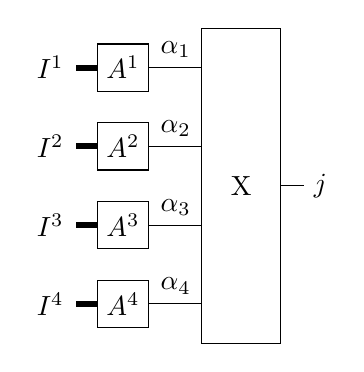
\begin{tikzpicture}[baseline=0.5]
        \draw (0,2.5)-- (0,-1.5) -- (1,-1.5)-- (1,2.5) -- cycle;

        \node[draw=none] (x)  at (0.5,0.5) {X};

        \node[draw, minimum size=0.6cm] (n1)  at (-1,2) {$A^1$};
        \node[draw, minimum size=0.6cm] (n2)  at (-1,1) {$A^2$};
        \node[draw, minimum size=0.6cm] (n3)  at (-1,0) {$A^3$};
        \node[draw, minimum size=0.6cm] (n4)  at (-1,-1) {$A^4$};

        \draw (n1) -- node [above] {$\alpha_1$} (0,2);
        \draw (n2) -- node [above] {$\alpha_2$} (0,1);
        \draw (n3) -- node [above] {$\alpha_3$} (0,0);
        \draw (n4) -- node [above] {$\alpha_4$} (0,-1);

        \draw[line width=0.75mm] (n1) -- ++(-0.6,0) node [left] {$I^1$};
        \draw[line width=0.75mm] (n2) -- ++(-0.6,0) node [left] {$I^2$};
        \draw[line width=0.75mm] (n3) -- ++(-0.6,0) node [left] {$I^3$};
        \draw[line width=0.75mm] (n4) -- ++(-0.6,0) node [left] {$I^4$};

        \draw (1,0.5) -- (1.3,0.5)  node [right] {$j$} ;

    \end{tikzpicture} }

\def \blockct { 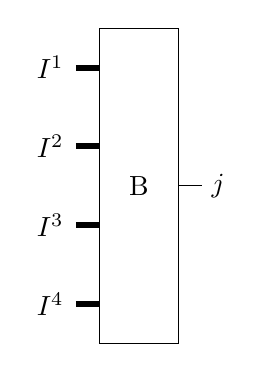
\begin{tikzpicture}[baseline=3]
        \draw (0,2.5)-- (0,-1.5) -- (1,-1.5)-- (1,2.5) -- cycle;

        \node[draw=none] (x)  at (0.5,0.5) {B};

        \draw[line width=0.75mm] (-0.3,2)  node [left] {$I^1$}  -- (0,2) ;
        \draw[line width=0.75mm] (-0.3,1)  node [left] {$I^2$} -- (0,1);
        \draw[line width=0.75mm] (-0.3,0)  node [left] {$I^3$} -- (0,0);
        \draw[line width=0.75mm] (-0.3,-1)  node [left] {$I^4$} -- (0,-1);

        \draw (1,0.5) -- (1.3,0.5)  node [right] {$j$} ;

    \end{tikzpicture} }

Now that it is clear how  the construction works, we focus on how to solve them numerically. Let's focus on the block $X=O^{1 1 1 1}$ from \cref{crosssolve}. The involved tensor are reshaped and reordered to bring it in the following form
\begin{equation}
    \epsilon = \vcenter{\hbox{ \pepoct }} - \vcenter{\hbox{  \blockct }} . \label{extract_x}
\end{equation}
Here $B$ is the exponentiated Hamiltonian the + geometry minus the contraction of all previous added blocks. $\epsilon$ is the residual error, and should be zero up to machine precision when the solver is finished. Solving this equation by inverting the matrices $A^i$ separately results in numerical unstable results, due to the ill conditioned chains. In practice this instability starts happening at virtual level 2. Taking the pseudoinverse of the tensor product  $A = A^1 \otimes A^2 \otimes A^3 \otimes A^4$  resolves the problem, but is  computationally too expensive. The problem is resolved by taking the SVD decomposition of each matrix $A^i = U^i \Sigma^i V^{i \dagger}$. The unitary matrices are inverted by taking the Hermitian transpose, and the sparse matrix $\Sigma = \Sigma^1 \otimes \Sigma^2 \otimes \Sigma^3 \otimes \Sigma^4$ is pseudoinverted.

\subsubsection{Nonlinear Solver}
A nonlinear solver takes steps in the direction that lowers the residual error $\epsilon$. This procedure can be sped up if the gradient is known. Inspection of \cref{extract_x} shows that the derivative  $\frac{\partial  \epsilon_{I^1 I^2 I^3 I^4 j }  }  { X_{\alpha_1 \alpha_2 \alpha_3 \alpha_1 } }   = A_{I^1 I^2 I^3 I^4 \alpha_1 \alpha_2 \alpha_3 \alpha_4 j } $. Or more simply contraction of the network but with X removed. This can be extended to more complex situation with the chain rule.
\subsection{other}

\begin{itemize}
    \item symmmetry
    \item truncation
    \item contraction
\end{itemize}

\subsubsection{Truncation}
The highest virtual level can be truncation in bond dimension. Introducing a block to solve a chain longer than the last exactly solved blocks leads to diverging results

\section{Results}
The cluster expansions are tested in 2 ways. In 1D and 2D, the error $\epsilon$ is calculated by comparing the contracted PEPO against the exact exponential.

\subsection{Exact exponentials}
\begin{figure}[h!]
    \center
    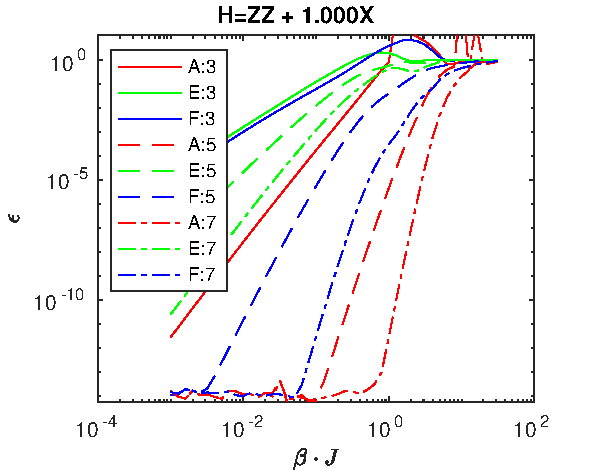
\includegraphics[width=\linewidth]{../Figuren/benchmarking/t_ising_small.pdf}
    \caption{Comparison type A, E and F for Transversal Ising. Error evaluated on cyclic chain. }
    \label{fig:benchmark:tising}
\end{figure}

In 1D, the error is calculated on a cyclic system of 11 sites. The results are shown in \cref{fig:benchmark:tising}. All the cluster expansion get better with increasing order. Type A outperforms the other 2 types by quite some margin. This conclusion is also true for the Heisenberg model and random 2 site Hamiltonians. The results in 2D show a similar trend. The error in 2D is of the same order of magnitude. The plaquette term \cref{tikzfig:plaquetter} is needed, the extensions are optional. The results show that real time evolution ($t = - i \beta$) also performs well.

\subsection{2D Transversal Ising}

A cluster expansion of order 5 with loops is used to simulate the phase transition of the transversal Ising model at g=0 (classical) and g=2.5. The simulated magnetisation $ \braket{m}$ and the data collapse of m, entropy $S$ and correlation length $\xi$ for g=2.5 is shown in \cref{fig:phase:g25:zoomed}. $\delta$ is a measure for the size of the system. \Cref{fig:phase:g25:zoomed} shows a very clear data collapse. For g=0, the fitted critical temperature $T_c = 2.691(9)$. Onsager's analytical solution is $T_c = 2.69185$. For $g=2.5$, the fitted value $T_c=1.2736(6)$ agrees well with values from literature, e.g. $T_c=1.2737(2)$ obtained with a competing tensor network technique and $T_c=1.2737(6)$ obtained with quantum Monte Carlo. \cite{Czarnik2019} Higher precision can be achieved with cluster expansions of higher order.

\begin{figure}[h!]
    \center
    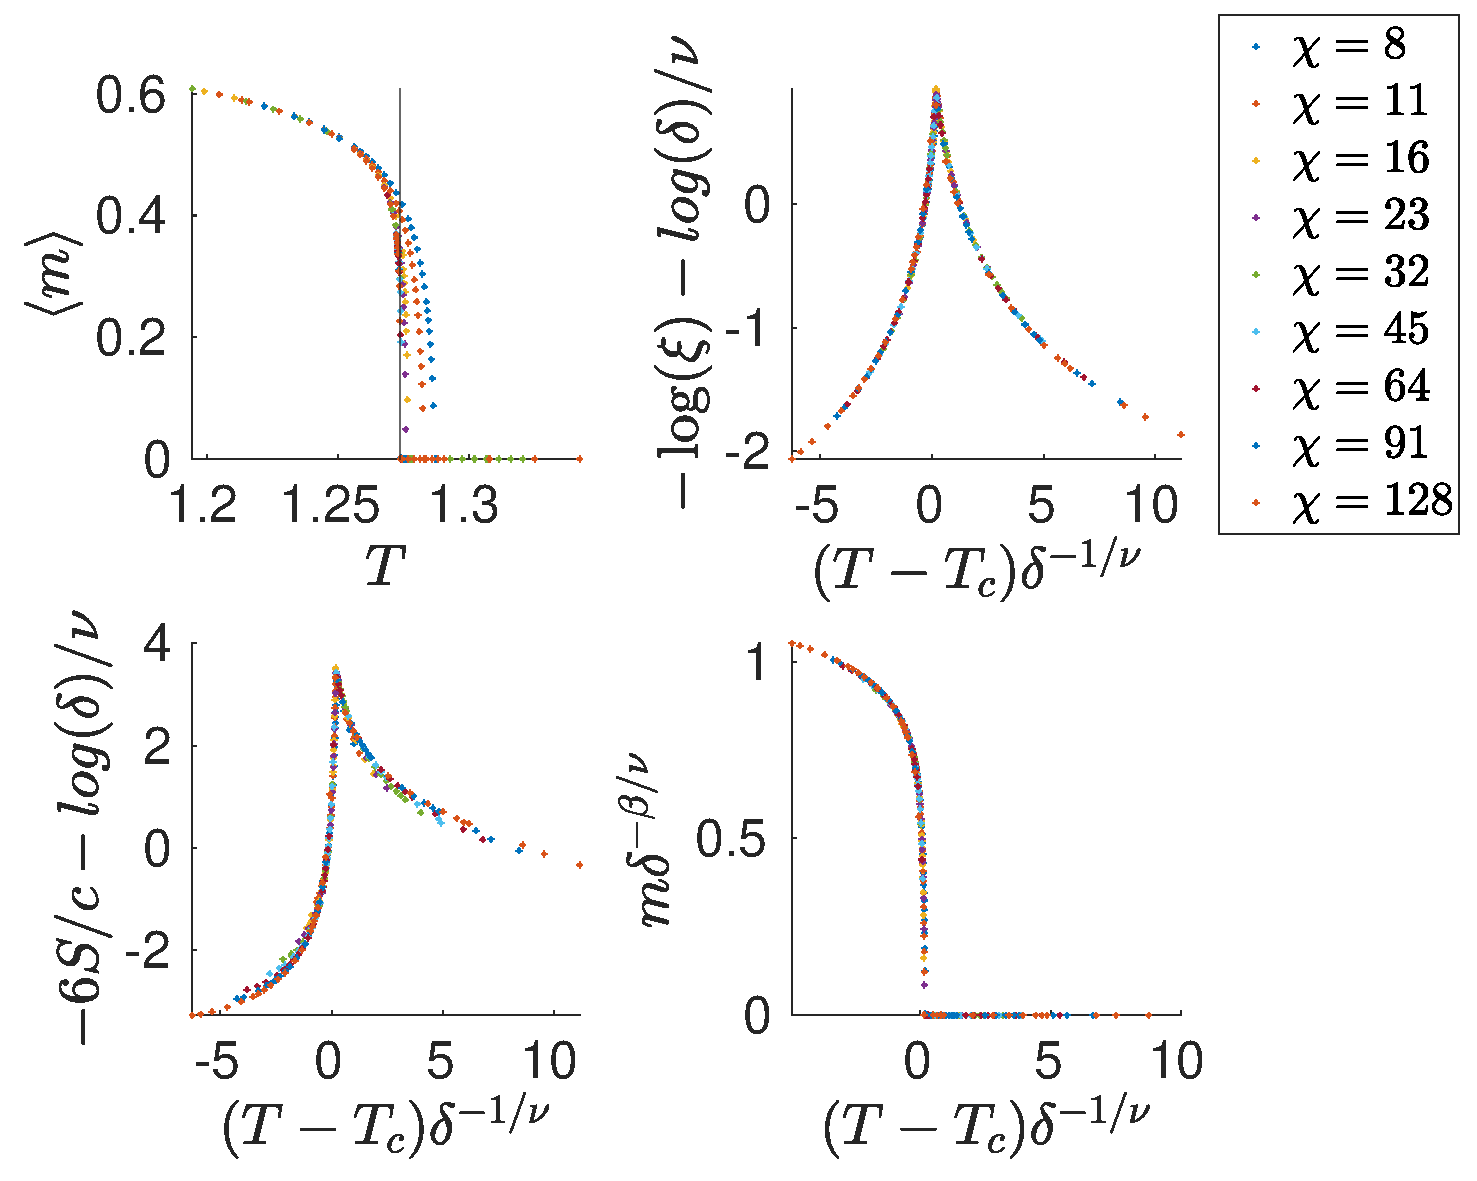
\includegraphics[width=\linewidth]{../Figuren/phasediag/g25/zoomed_small.pdf}
    \caption{ Data collapse for $g=2.5$ phase transition of transversal Ising Model. Data points are taken from $T \in \left[ T_c -0.08, T_c +0.08 \right]$. }
    \label{fig:phase:g25:zoomed}
\end{figure}

\section{Outlook}

The results agree well with exact exponentiation and with critical values from literature, proving that these cluster expansion can compete with other methods.  \todo{more}

With current methods,
\bibliographystyle{plain}
\bibliography{../bib.bib}
\end{document}
